\documentclass{article}
\usepackage[utf8]{inputenc}
\usepackage{algorithm}
\usepackage{algpseudocode}
\usepackage{graphicx}
\usepackage[parfill]{parskip}
\usepackage{hyperref}
\usepackage{amsmath}
\usepackage{amsfonts}

\setlength{\parindent}{0pt}
\setlength{\parskip}{8pt}

\title{Reinforcement Learning}
\author{Zexuan Meng}

\begin{document}

\maketitle

\section{Monte Carlo Methods}

Monte Carlo methods in RL are a class of algorithms that rely on \hyperref[sec:repeated-random-sampling]{\emph{repeated random sampling}} and average the sample returns. They are used to estimate the value functions and discover optimal policies. Monte Carlo methods are used when the agent's environment is modeled as a Markov Decision Process (MDP), but the agent does not have complete knowledge of the environment. In particular, it does not know the transition probabilities and rewards for each state. Instead, it learns from experience by sampling episodes of experience from the environment. The \emph{experience}, sequences of states, actions, and rewards, are the only information required to apply Monte Carlo methods. We define Monte Carlo methods only for episodic tasks. That is, the experience is divided into episodes and all episodes will eventually terminate.

To conclude, the key characteristics of Monte Carlo methods are:

\begin{itemize}
    \item \textbf{Model-free}: Monte Carlo methods do not require a model of the environment's dynamics.
    \item \textbf{Episodic-based}: Monte Carlo methods learn from complete episodes. They do not \hyperref[sec:bootstrapping]{bootstrap}.
    \item \textbf{Sampled returns}: Monte Carlo methods use the \emph{empirical mean return} rather than the \emph{expected return} to estimate the value functions.
\end{itemize}

\subsection{Basic concept for Monte Carlo methods}

\subsubsection{Repeated random sampling}\label{sec:repeated-random-sampling}

Repeated random sampling is a statistical technique where subsets, or samples, are taken from a larger population or dataset while each sample is selected randomly. The idea behind repeated random sampling is to obtain a representative subset of the larger population, which can be analyzed to infer the properties of the entire population. Each sample should be selected using a process that gives every possible sample an \emph{equal} chance of being chosen.

Here are some sampling techniques that may be employed:

\begin{itemize}
    \item \textbf{Simple random sampling}: Every member of the population has an equal chance of being included in the sample.
    \item \textbf{Stratified sampling}: The population is divided into mutually exclusive groups, called strata, and random samples are taken from each stratum.
    \item \textbf{Cluster sampling}: The population is divided into mutually exclusive groups, called clusters, and then all members of the clusters are included in the sample.
\end{itemize}

\subsubsection{Bootstrapping in Monte Carlo methods}\label{sec:bootstrapping}

Bootstrapping refers to the process of updating estimates based on other current estimates rather than waiting until the final outcome is known.

Monte Carlo methods \emph{do not} bootstrap. Because they update the value function only at the end of an episode, based on the entire sequence of observed rewards from the episode. They use the total accumulated reward from the current state until the end of the episode to update the value function. In this case, the value function for a certain state is updated based on the \emph{actual rewards} rather than the \emph{expected rewards}.

\subsection{Monte Carlo Prediction}

First, we would like to learn the state-value function for a given policy with Monte Carlo methods. The value of a certain state, the expected return, is the expected cumulative future discounted reward starting from that state. To estimate from experience, we can simply average the returns observed after visits to that state. \emph{As more returns are observed, by the law of large numbers, the average should converge to the expected value.} This idea is the basis of Monte Carlo prediction.

Each occurrence of state $s$ in an episode is called a \emph{visit} to $s$.
\begin{itemize}
    \item \textbf{First-visit}: The first time-step $t$ that state $s$ is visited in an episode.
    \item \textbf{Every-visit}: Every time-step $t$ that state $s$ is visited in an episode.
\end{itemize}

First-visit Monte Carlo methods estimate the value of a state as the average of the returns following first visits to that state. Every-visit Monte Carlo methods estimate the value of a state as the average of the returns following all visits to that state. The two methods converge to the true value function as the number of visits to each state goes to infinity. Notice that there is no guarantee to pass by all states. Here we only focus on first-visit Monte Carlo methods.

\begin{algorithm}
    \caption{First-visit MC prediction, for estimating $V \approx v_\pi$}\label{alg:FV-MC-V}
    \begin{algorithmic}
        \State Input: a policy $\pi$ to be evaluated
        \State Initialize:
        \State \hspace{\algorithmicindent} $V(s) \in \mathbb{R}$, arbitrarily, for all $s \in \mathcal{S}$
        \State \hspace{\algorithmicindent} $Returns(s) \leftarrow$ an empty list, for all $s \in \mathcal{S}$
        \Loop{ for each episode}
        \State Generate an episode following $\pi$: $S_0, A_0, R_1, S_1, A_1, R_2, \dots, S_{T-1}, A_{T-1}, R_T$
        \State $G \leftarrow 0$
        \For{$t = T-1, T-2, \dots, 0$}
        \State $G \leftarrow \gamma G + R_{t+1}$
        \If{$S_t$ not in $S_0, S_1, \dots, S_{t-1}$}
        \State Append $G$ to $Returns(S_t)$
        \State $V(S_t) \leftarrow \text{average}(Returns(S_t))$
        \EndIf
        \EndFor
        \EndLoop
    \end{algorithmic}
\end{algorithm}

Detailed explanation of Algorithm~\ref{alg:FV-MC-V}:

Initialize:
\begin{itemize}
    \item $V(s)$: value function in state $s$.
    \item $Returns(s)$: total rewards in state $s$.
\end{itemize}

Loop for each episode:
\begin{itemize}
    \item Generate an episode: how we use the policy.
    \item $G$:  the total return from the current state to the end of the episode.
    \item if $S_t$ not in $S_0, S_1, \dots, S_{t-1}$: check if it is the first visit to state $S_t$. This clause will ensure that we only count the first visit to state $S_t$.
    \item $V(S_t) \leftarrow \text{average}(Returns(S_t))$: the average here is the key idea of MC methods, the utilization of law of large numbers.
\end{itemize}

Now let's talk about why we did a backward loop in each episode to update the total return. The reason is very intuitive since the return $G_t$ from a state $S_t$ is the total discounted reward received from time $t$ \emph{onwards} until the end of the episode:

\begin{align*}
    G_t &= R_{t+1} + \gamma R_{t+2} + \gamma ^2 R_{t+3} + ... + \gamma ^{T-t-1} R_{T} \\
    &= R_{t+1} + \gamma G_{t+1}
\end{align*}

Since $R_T$ is the immediate reward provided by the terminal state, $G_T$ is always 0. In this case, $G_{T-1} = R_T + \gamma G_T = R_T$ and it's really easy to start at this point.

\begin{align*}
    G_{T-1} &= R_T + \gamma G_T = R_T\\
    G_{T-2} &= R_{T-1} + \gamma G_{T-1} = R_{T-1} + \gamma R_T\\
    G_{T-3} &= R_{T-2} + \gamma G_{T-2} = R_{T-2} + \gamma R_{T-1} + \gamma ^2 R_T\\
    &\vdots\\
    G_1 &= R_2 + \gamma G_2 = R_2 + \gamma R_3 + \gamma ^2 R_4 + ... + \gamma ^{T-2} R_T\\
    G_0 &= R_1 + \gamma G_1 = R_1 + \gamma R_2 + \gamma ^2 R_3 + ... + \gamma ^{T-1} R_T
\end{align*}

\begin{minipage}[c]{0.9\textwidth}
    Why can we do the calculation like this? Because the Monte Carlo diagram goes all the way to the end of the episode and there is no diversion. Another important fact about Monte Carlo methods is that the estimates for each state are independent. Above all, I think that's why we chose to start at the end of the episode to update the total return.
\end{minipage}
\hfill
\begin{minipage}[c]{0.1\textwidth}
    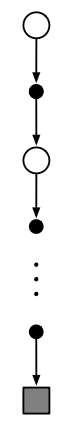
\includegraphics[height = 2.5\textwidth]{Figures/MC_diagram.png}
\end{minipage}

\subsection{Compare with Dynamic Programming}

Let's recall the Bellman equation for the optimal state-value function:

\[v_*(s) = \max_a\sum_{s', r} p(s',r|s,a) \left[ r + \gamma v_*(s')\right]\]

In Dynamic Programming, we need to know the \emph{transition matrix} as well as the \emph{reward system}, but it is not always the realistic condition. In reality, we may not know $p(s',r|s,a)$. In this case, we cannot compute $V(s)$. By adopting Monte Carlo methods, we play enough number of episodes of the game and extract the information needed.

In DP, we didn't play the game because we already knew the dynamics of the game, which is at each state we knew what are the probabilities of going to another state when we took certain actions, and we knew what the reward is going to be. In Monte Carlo methods, we don't know those data unless we play the game. That's the key difference between DP and MC methods.
\end{document}
